\documentclass{article}
\usepackage[fontsize=8pt]{fontsize}
\usepackage[utf8]{inputenc}
\usepackage{listings}
\lstset{
  basicstyle=\ttfamily,
  columns=fullflexible,
  frame=single,
  breaklines=true,
  postbreak=\mbox{\textcolor{red}{$\hookrightarrow$}\space},
}
\usepackage{lmodern} % for bold teletype font
\usepackage{minted}
\usepackage[autostyle=true]{csquotes}
%\usepackage{hyperref}
\usepackage[hidelinks]{hyperref}
\usepackage[T1]{fontenc}
\usepackage[english]{babel}
\usepackage[utf8]{inputenc}
\usepackage{setspace}
\usepackage{caption}
%\usepackage[margin=1.5cm]{geometry}
\usepackage{geometry}
\geometry{left=10mm,top=20mm, bottom=20mm, right=10mm}
\usepackage{float}
%\usepackage[nottoc,numbib]{tocbibind}
\usepackage{tocloft}
\usepackage{amsmath}
\usepackage{tabu}
\usepackage{float}
\usepackage{wrapfig}
\usepackage{multirow}
\usepackage{gensymb}
\usepackage{graphicx}
\usepackage{rotating}
\usepackage{subcaption}
\usepackage{tasks}
\usepackage{hyperref}
\usepackage{ragged2e}
\usepackage{subcaption}
\usepackage{wrapfig}
\usepackage{xcolor}
\usepackage{chemfig}
\usepackage{mhchem}
\DeclareCaptionType{equ}[][]
\captionsetup[equ]{labelformat=empty} 

\setlength{\parindent}{0cm}
\setcounter{secnumdepth}{5}
\setcounter{tocdepth}{5}
\onehalfspacing
\usepackage{fancyhdr}
\usepackage{etoolbox}
%\usepackage{biblatex}
\usepackage[
    backend=biber, 
    natbib=true,
    style=numeric,
    sorting=none
]{biblatex}
\addbibresource{myReferences.bib}
%\bibliographystyle{unsrt}


\pagestyle{fancy}
\fancyhf{}
\rhead{Final Exam 2022}
\lhead{ Enrico Turato - Processing and Analysis of Biological Data, BIOS14}
\lfoot{Blossoms \& Mountain Goats}
\cfoot{\thepage}
\rfoot{2023-JAN-13}

\newcommand{\listequationsname}{List of Equations}
\newlistof{myequations}{equ}{\listequationsname}
\newcommand{\myequations}[1]{%
\addcontentsline{equ}{myequations}{\protect\numberline{\theequation}#1}\par}
\setlength{\cftmyequationsindent}{1.5em}
\setlength{\cftmyequationsnumwidth}{2.3em}
\renewcommand{\cftequtitlefont}{\normalfont\Large\bfseries}

\begin{document}
        \Large
        \begin{center}
        \textbf{Double Dataset Analysis: Two-Way ANOVA for the Win}
               
        \Large
        Processing and Analysis of Biological Data, BIOS14
        
        \large
        Enrico Turato, Final Exam 2022, 2023-JAN-13
        \end{center} 
The exam comprises two parts. Each part includes the 
analysis of a dataset, for which I have chosen my own research questions that I answered through statistical analysis of the available data.\\ 
Visit Github to have access to the repository containing the code (also inserted in \autoref{Appendix}) (and in general all the other files related) used for this small analysis exercise: \url{https://github.com/EnricoTurato/Final_Exam_BIOS14_2022.git}.
%\begin{titlepage}
    \begin{center}
        \begin{figure}[H]
            \centering
            
\includegraphics[scale=0.3]{LundUniversity_C2line_RGB.png}
        \end{figure}
        
        \vspace*{1 cm}
        
        \Huge
        \textbf{Blossoms Dataset}
        
        \huge
        \vspace{0.4cm}
        Processing and Analysis of Biological Data\\
        BIOS14
        
        \LARGE
        \vspace{2cm}
        Enrico Turato\\
        
        \LARGE
        \vspace{2cm}
        Mid Term Exercise\\
        
        \Large
        \vspace{3 cm}
        2022-NOV-28
        
        \vspace{1cm}

    \end{center}
\end{titlepage}
%\tableofcontents
%\clearpage
%\listoffigures
%\listoftables
%\listofmyequations
%\clearpage
\section{Part 1: Blossoms in Greenhouse}

\subsection{Background and first dataset description}

I worked with data from an experiment in which \emph{Dalechampia Plants}, from two populations each of two species (“S” and “L”) were exposed to either dry or wet experimental conditions in a greenhouse (treatment). Blossom traits were measured on blossoms in early bisexual condition. The data comprise of many variables among which the important ones for my analysis are the following.
sp: species ID; treat: treatment (dry or wet); LBL: lower bract length [mm] and  UBL: upper bract length [mm]. The upper and lower bract lengths are averages of the lengths from the bract base to the tip of the three lobes, and their function is similar to petals in flower, acting as advertisement.

\subsection{Scientific questions and analysis methods chosen}
It is interesting to assess the effects of two experimental factors, or categorical variables (in this case the chosen two are "sp" and "treat", meaning the plants species, either S or L and the treatment, either wet or dry), plus their potential interaction, on some chosen response variables that in this case are the lower bract length (LBL) and the upper one (UBL).
Following the philosophy of an effect size-centered approach and given the presence of two factors, or categorical variables among all the others, I decided to focus on a two-way ANOVA-type of analysis. So a two-way ANOVA has been performed two times, one for the first mentioned response variable (m = lm(dat\$LBL$\sim$species*treatment),
anova(m)) and one for the second one (m = lm(dat\$UBL$\sim$species*treatment),
anova(m)). At the end, estimates as percentage values are given and the main parameters from the ANOVA analysis have been reported.

\subsection{Results and Conclusions}
First of all I created four sub-dataset starting from the complete one, just by filtering, in order to group data by the treatments and by species and to observe the distributions of LBL and UBL through histograms to get a rough idea of the values from a quantitative point of view before moving to the ANOVA. The four dataset contained "wet-plants only", "dry-plants only", "L-plants only" and "S-plants only". The results are the following. \autoref{fig:histolbl2} for LBL and \autoref{fig:histoubl2} for UBL.
\iffalse
\begin{figure}[H]
\centering
  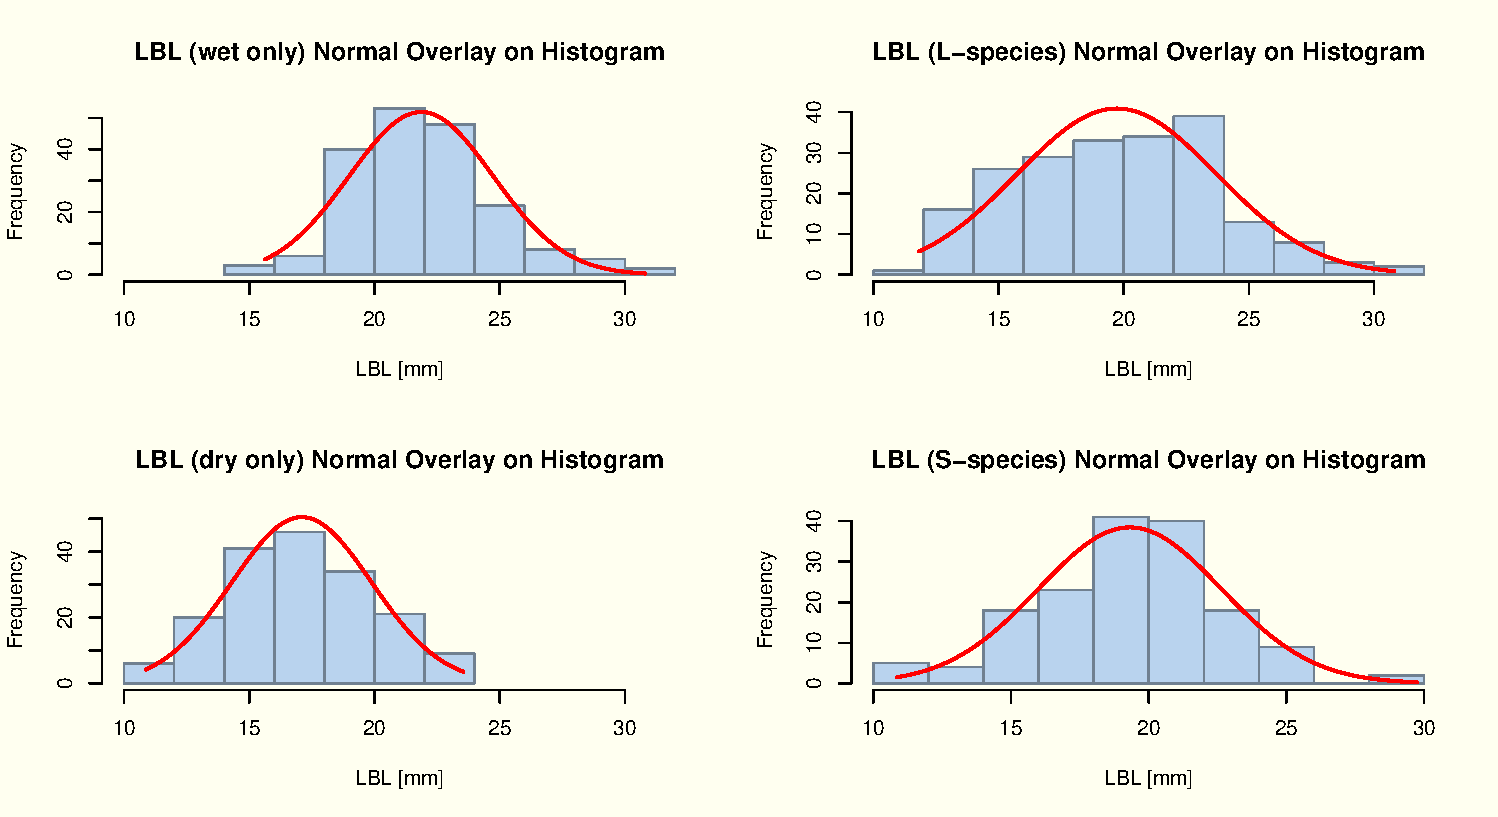
\includegraphics[scale=0.5]{histograms_lbl.pdf}
\caption{LBL data: top left, the histogram from the "wet" data; bottom left, the histogram from the "wet" data; top right, the histogram from the "L-species" data; bottom right, the histogram from the "S-species" data. A normal distribution overlay is on all four of them for reference.}
  \label{fig:histolbl}
\end{figure}
\begin{figure}[H]
\centering
  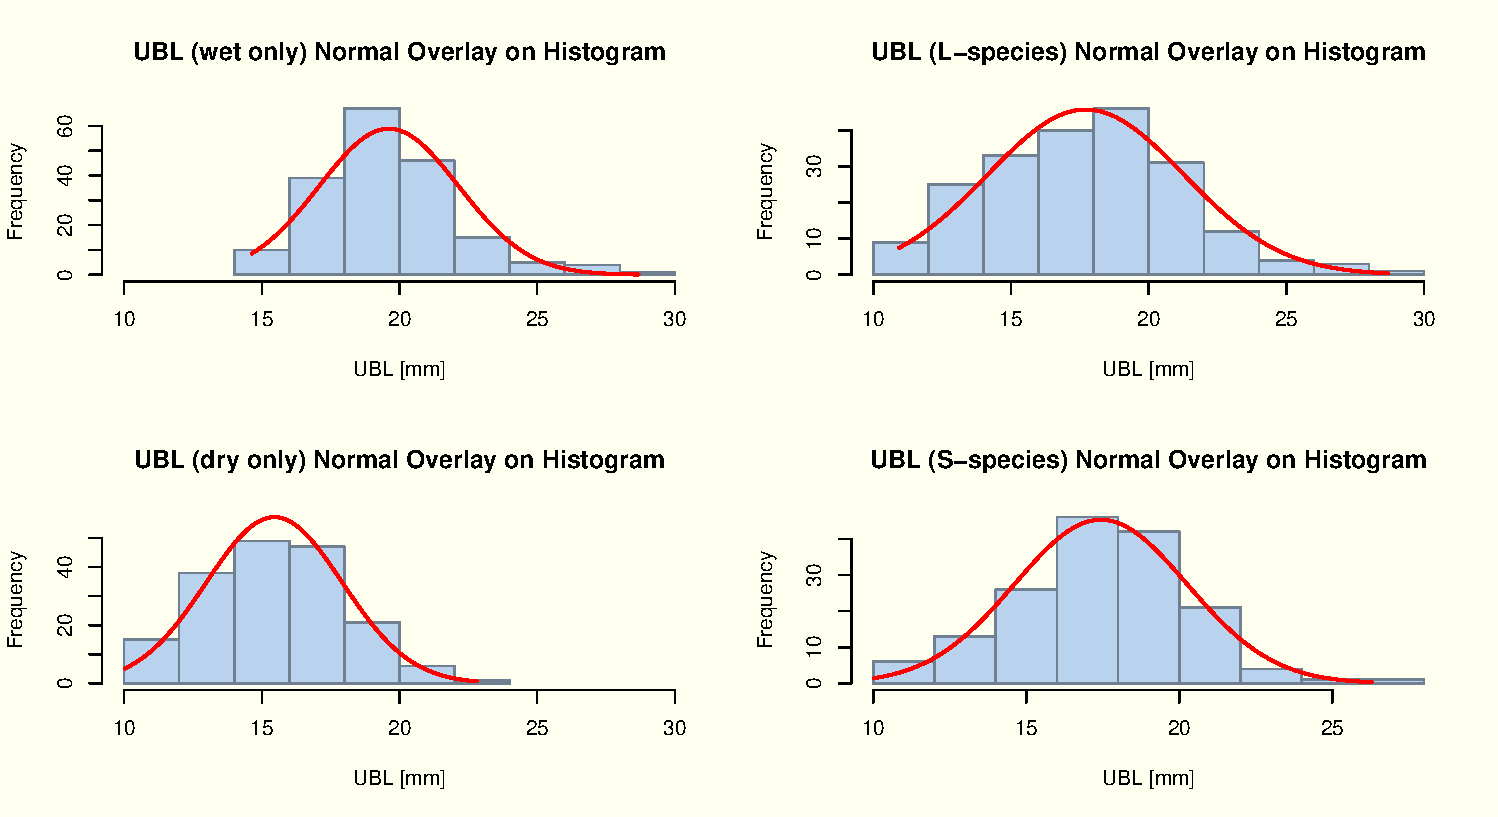
\includegraphics[scale=0.5]{histograms_ubl.pdf}
\caption{UBL data: top left, the histogram from the "wet" data; bottom left, the histogram from the "wet" data; top right, the histogram from the "L-species" data; bottom right, the histogram from the "S-species" data. A normal distribution overlay is on all four of them for reference.}
  \label{fig:histoubl}
\end{figure}
\fi
\begin{figure}[H]
     \centering
     \caption{True for both the left image and for the right one: top left, the histogram from the "wet" data; bottom left, the histogram from the "wet" data; top right, the histogram from the "L-species" data; bottom right, the histogram from the "S-species" data. A normal distribution overlay is on all four of them for reference.}
     \subfloat[][LBL histograms]{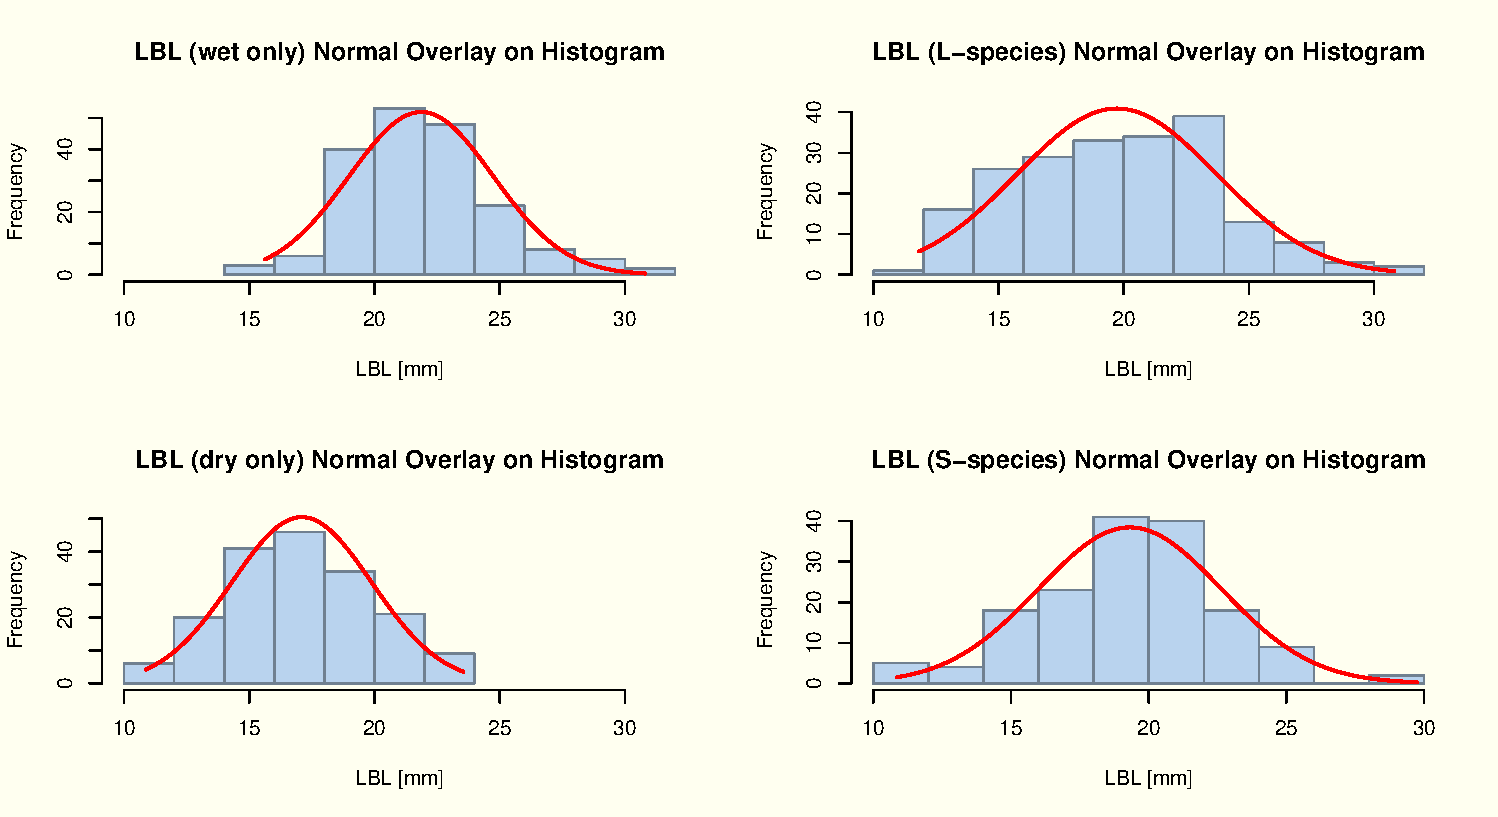
\includegraphics[scale = 0.365]{histograms_lbl.pdf}\label{fig:histolbl2}} \qquad
     \subfloat[][UBL histograms]{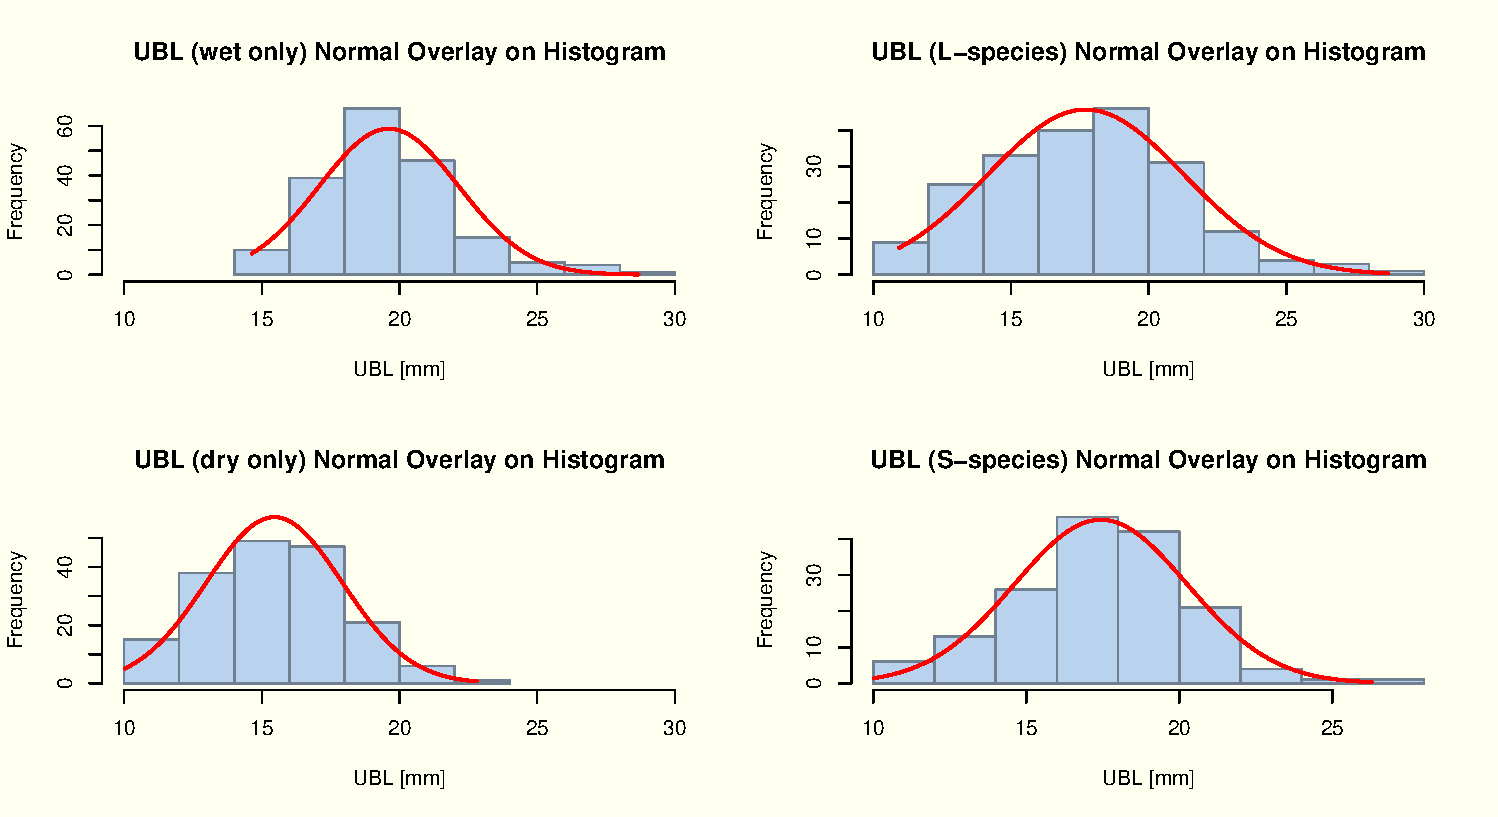
\includegraphics[scale = 0.365]{histograms_ubl.pdf}\label{fig:histoubl2}}
\end{figure}
I then checked the distribution of data also with some boxplots, see \autoref{fig:boxi1} and \autoref{fig:boxi2}.
\begin{figure}[H]
     \centering
     \caption{True for both the left image and for the right one: on the left, boxplots showing the data distribution of the LBL depending on the species. On the right boxplots showing the data distribution of the LBL depending on the treatment.}
     \subfloat[][LBL boxplots]{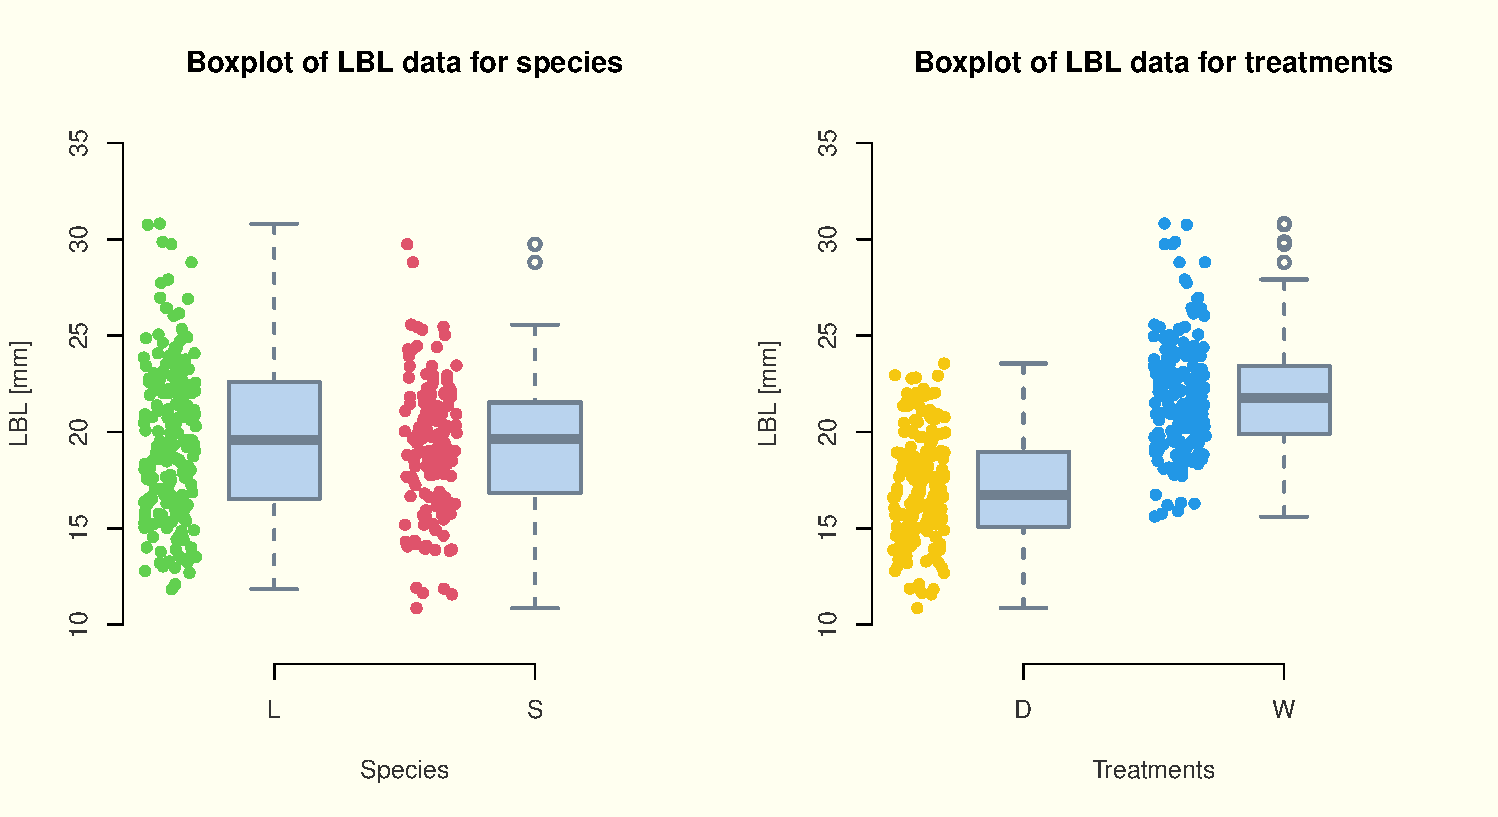
\includegraphics[scale = 0.365]{boxplots_lbl.pdf}\label{fig:boxi1}} \qquad
     \subfloat[][UBL boxplots]{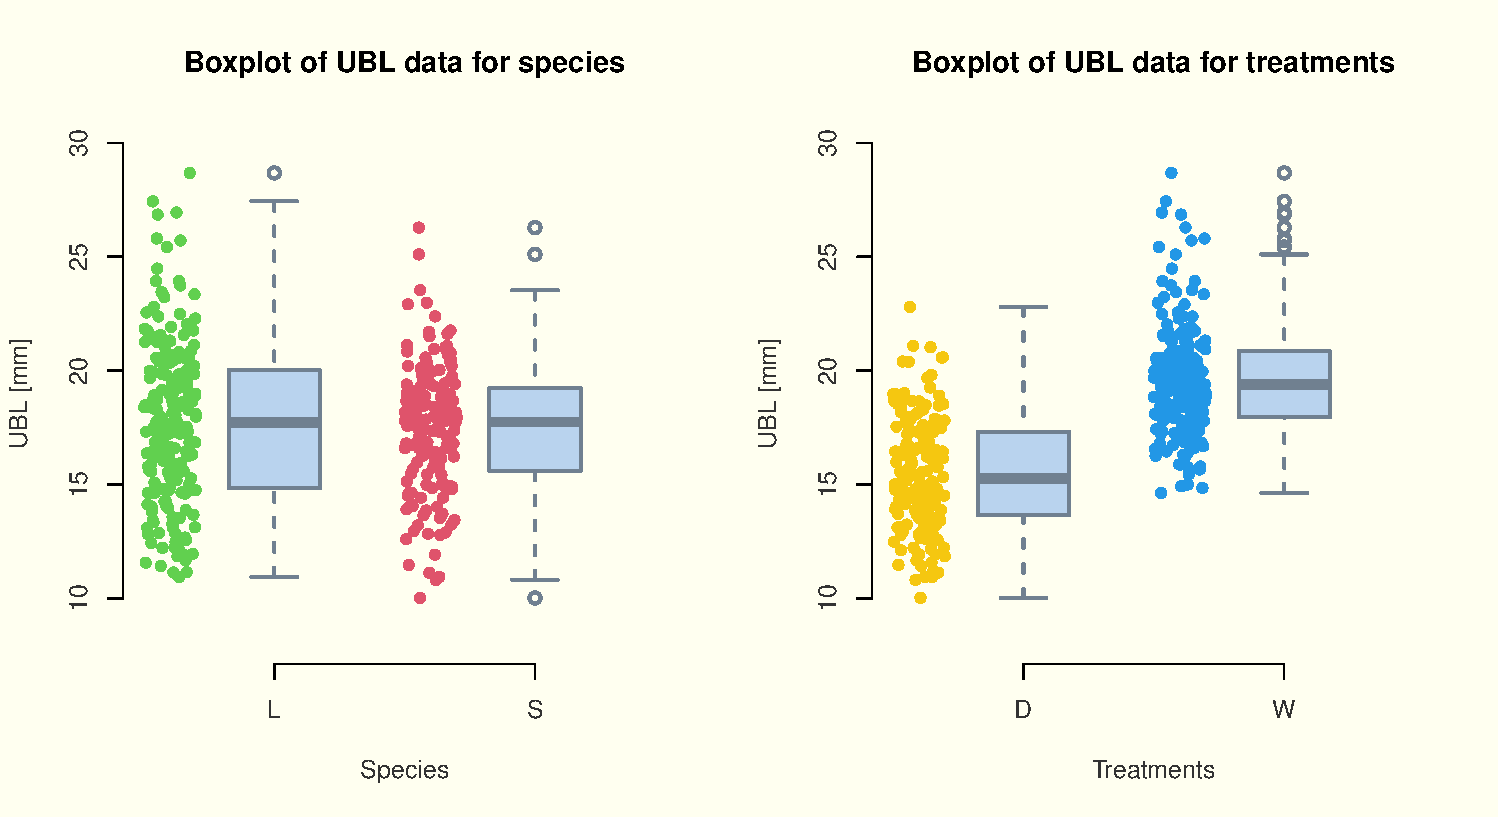
\includegraphics[scale = 0.365]{boxplots_ubl.pdf}\label{fig:boxi2}}
\end{figure}
\iffalse
\begin{figure}[H]
\centering
  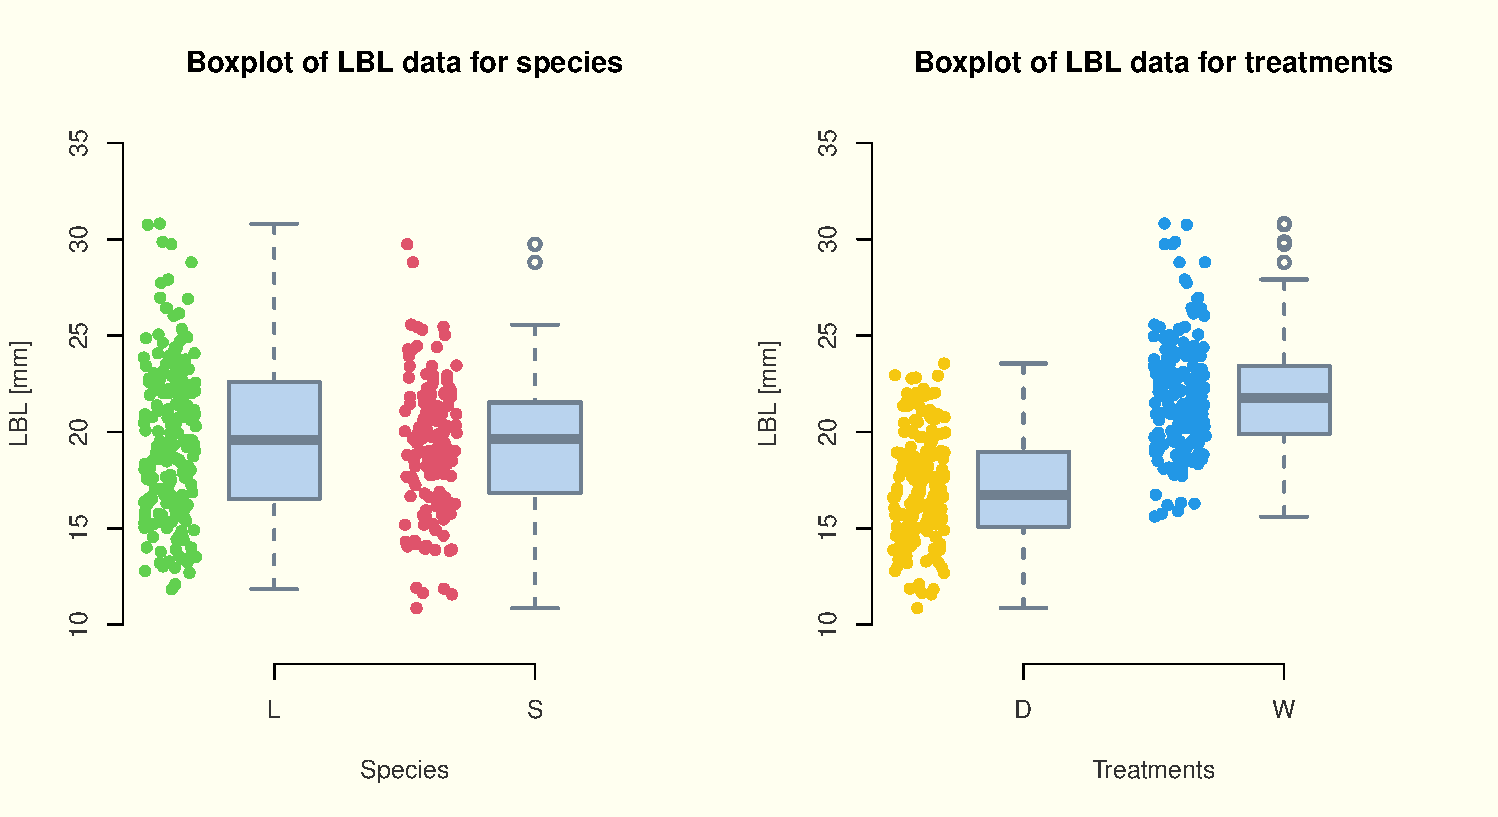
\includegraphics[scale=0.5]{boxplots_lbl.pdf}
\caption{On the left, boxplots showing the data distribution of the LBL depending on the species. On the right boxplots showing the data distribution of the LBL depending on the treatment.}
  \label{fig:boxi1}
\end{figure}
\begin{figure}[H]
\centering
  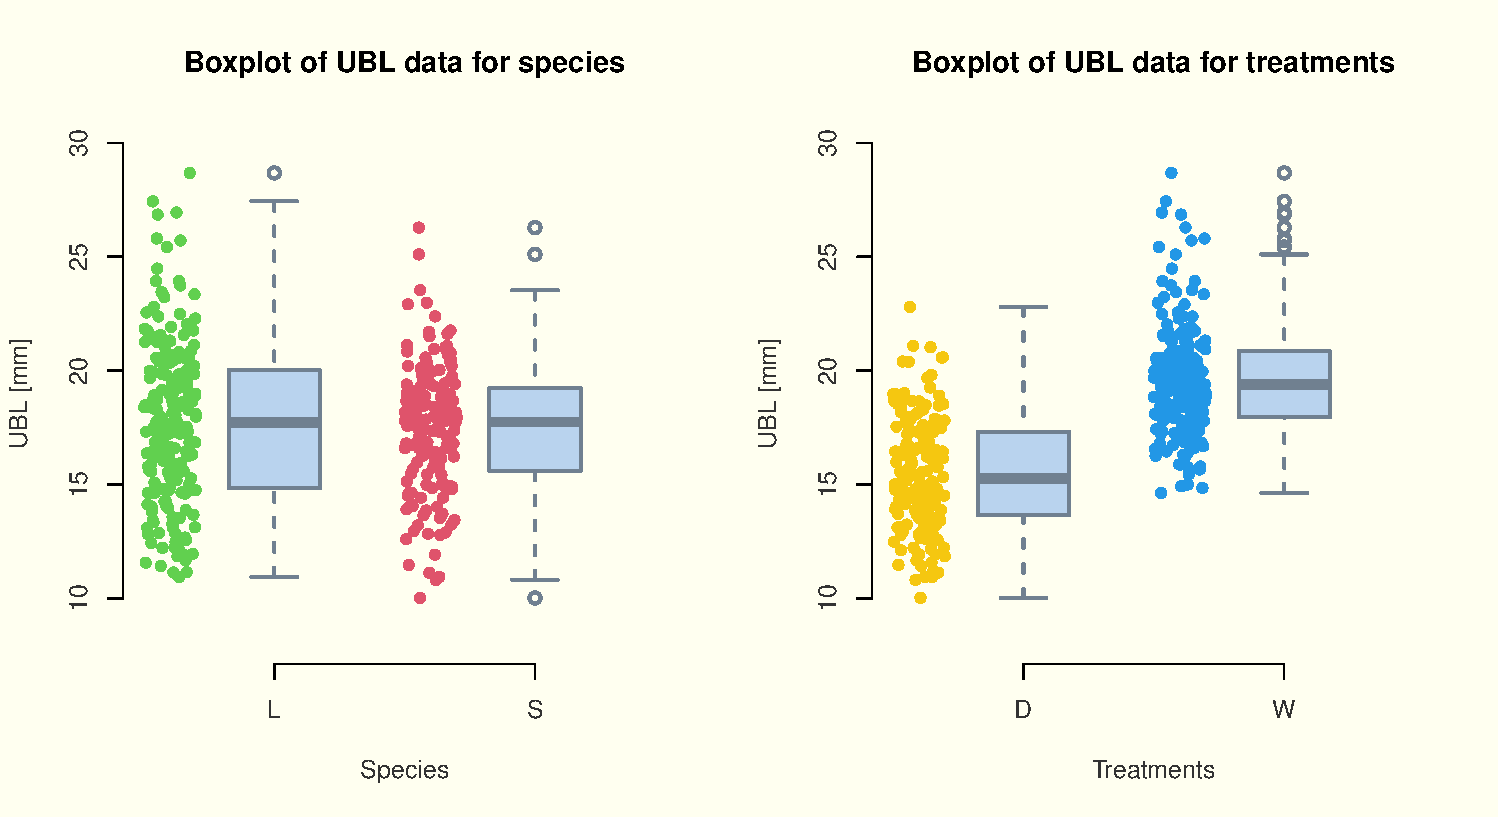
\includegraphics[scale=0.5]{boxplots_ubl.pdf}
\caption{On the left, boxplots showing the data distribution of the UBL depending on the species. On the right boxplots showing the data distribution of the UBL depending on the treatment.}
  \label{fig:boxi2}
\end{figure}
\fi
Next, to get some estimates, I performed the two-way ANOVA analysis. 
First of all, after computing the means and errors for LBL data and UBL data, see \autoref{tab:aovi1} left and right respectively, from a graphical point of view I obtained \autoref{fig:aovi1}.
\begin{table}[!htb]
    \caption{Means [mm] (above) and standard errors [mm] (below) for both LBL (left side) and UBL (right side).}
    \label{tab:aovi1}
    \begin{minipage}{.5\linewidth}
      \centering
\begin{tabular}{c c c} 
 \hline
/ & Dry & Wet   \\  
 \hline
 L-species &17.05&22.55 \\
 S-species &17.15&21.09  \\
 \hline
 \hline
/ & Dry & Wet   \\  
 \hline
 L-species &0.27&0.30 \\
 S-species &0.34&0.27  \\
 \hline
\end{tabular}
    \end{minipage}%
    \begin{minipage}{.5\linewidth}
      \centering
\begin{tabular}{c c c} 
 \hline
/ & Dry & Wet   \\  
 \hline
 L-species &15.37&20.20 \\
 S-species &15.57&18.96  \\
 \hline
 \hline
/ & Dry & Wet   \\  
 \hline
 L-species &0.25&0.27 \\
 S-species &0.29&0.23  \\
 \hline
\end{tabular}
    \end{minipage} 
\end{table}

\begin{figure}[H]
\centering
  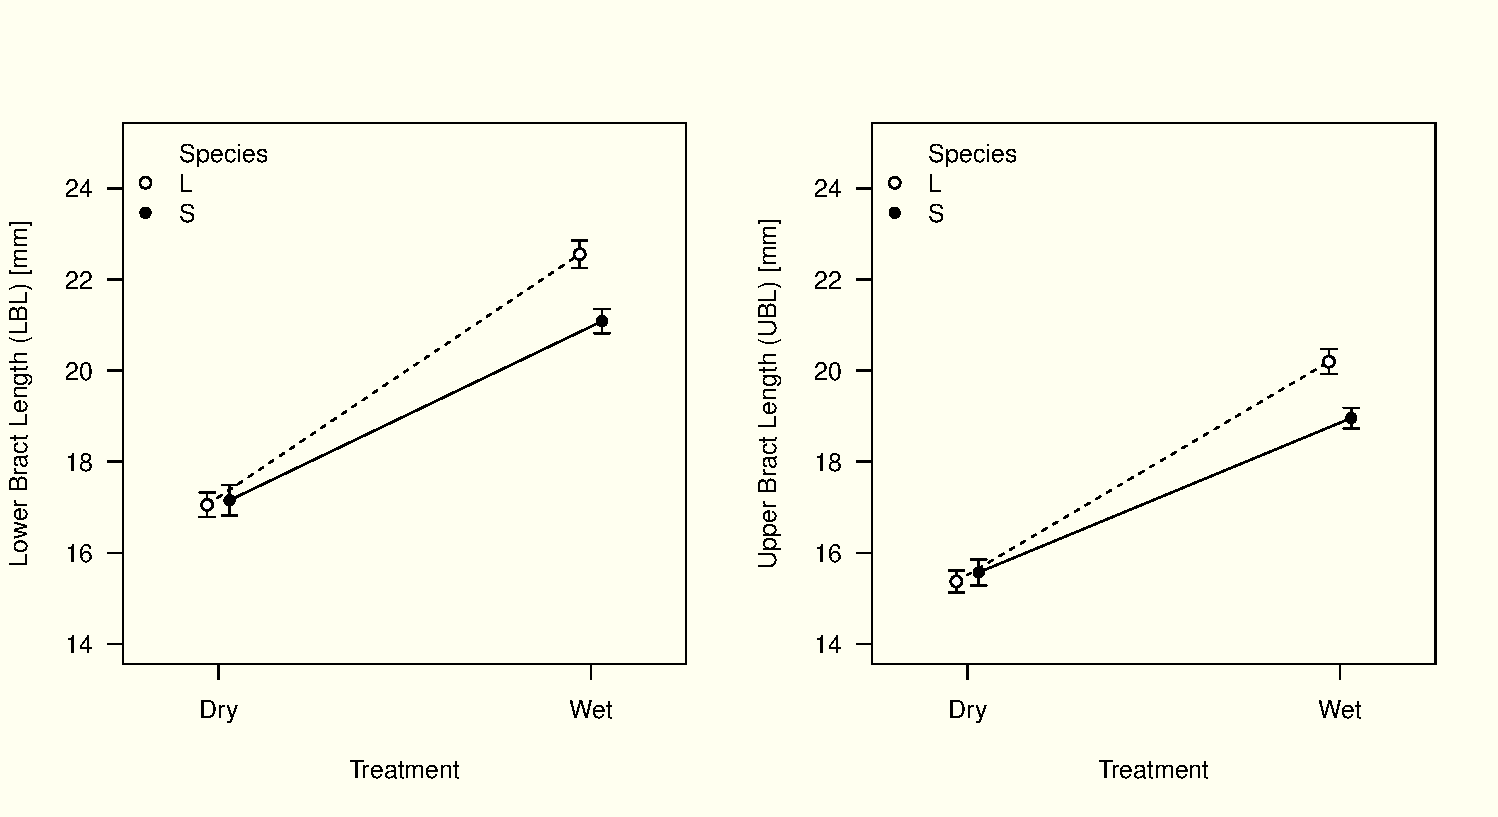
\includegraphics[scale=0.5]{anova_lbl.pdf}
\caption{Plots giving a graphical idea of the size effect for the two-way ANOVA analysis performed for both the LBL and UBL when considering species and treatment type as factors.}
  \label{fig:aovi1}
\end{figure}

Talking about the LBL (UBL), to interpret the results, by considering the ANOVA table, one sees that there are detectable effects of mainly treatment compared to the species contribution: more variance is indeed explained by treatment (based on the larger sum of squares: $\approx$ 2101 (1594) and $\approx$ 15 (7), respectively). Furthermore, the effects of species and treatment are not independent, as indicated by enough statistical support (P $\approx$ 0.008 (0.006), F$_{1,360}$ $\approx$ 7 (8)). The variance explained by the interaction term is indeed not negligible when compared to the above mentioned ones (sum of squares: $\approx$ 55 (46)).\\
\iffalse
Talking about the UBL there are also detectable effects of mainly treatment compared to the species contribution: more variance is indeed explained by treatment (based on the larger sum of squares: $\approx$ 1594 and $\approx$ 7, respectively). Furthermore, the effects of species and treatment are not independent, as indicated by enough statistical support (P $\approx$ 0.006, F$_{1,360}$ $\approx$ 8). The variance explained by the interaction term is indeed not negligible when compared to the above mentioned ones (sum of squares: $\approx$ 46).\\
\fi
To quantify the effect size in both cases, I computed the mean LBL and UBL for each treatment and species from \autoref{tab:aovi1} by working first on columns and then on rows. Based on this, I can finally say the following.\\
The mean LBL (UBL) (taking the mean between L-species and S-species) was 21.6\% (21\%) shorter when considering plants with a dry treatment than when having a wet one (mean LBL (UBL) = 17.10 (15.47) mm and 21.82 (19.58) mm, respectively, F$_{1,360}$ $\approx$ 269 (261), P << 0.00001, \autoref{fig:aovi1}).
When considering the effect of species instead, the mean LBL (UBL) for S-species (taking the mean between dry treatment and wet treatment) was only 3.5\% (2.9\%) shorter with respect to L-species (mean LBL (UBL) = 19.12 (17.26) mm and 19.80 (17.78) mm, respectively, F$_{1,360}$ $\approx$ 2 (1), P > 0.16 (0.28), \autoref{fig:aovi1}).
The difference in LBL (UBL) between treatments was noticeable between the two species as correctly showed by the small above mentioned statistical support for the contribution of the interaction term (24.4\% (23.9\%) vs. 18.6\% (17.9\%), respectively L and S species; P = $\approx$ 0.008 (0.006)).\\
\iffalse
The mean UBL (taking the mean between L-species and S-species) was 21\% shorter when considering plants with a dry treatment than when having a wet one (mean UBL = 15.47 and 19.58 mm, respectively, F$_{1,360}$ $\approx$ 261 , P << 0.00001, \autoref{fig:aovi1}).
When considering the effect of species instead, the mean UBL for S-species (taking the mean between dry treatment and wet treatment) was 2.9\% shorter with respect to L-species (mean UBL = 17.26 and 17.78 mm, respectively, F$_{1,360}$ $\approx$ 1, P > 0.28, \autoref{fig:aovi1}).
The difference in UBL between treatments was noticeable between the two species as correctly showed by the small above mentioned statistical support for the contribution of the interaction term (23.9\% vs. 17.9\%, respectively L and S species; P $\approx$ 0.006).\\
\fi
All things considered, from the analysis of this particular dataset with the specified methods, it has been shown that treatment is affecting more the bracts length (when wet the bracts are longer in mean) than the existence of two species of plants (S and L) for both LBL and UBL. It has been shown also that there seems to be a non negligible interaction between the treatment and the species even though small.

\section{Part 2: Mountain Goats}
The following dataset comprises measurements of horn length and body mass of mountain goats. The data included many variables among which the chosen one for the analysis were the following.
Sex: M/F; hornL: length of the left horn in mm; hornR: length of the right horn in mm; mass: body mass in kg; density: population density at birth, low / high. 

\subsection{Scientific questions and analysis methods chosen}
Following the philosophy of an effect size-centered approach and given the presence of two factors, or categorical variables among all the others (meaning "sex" and population "density" at birth), it is quite understandable to be curious about the possible relation between such factors and the influence on certain physical response variables from a quantitative point of view such as the horn length and the body mass.
I decided to focus on a two-way ANOVA-type of analysis in order to assess the effects of each experimental factor (categorical variables) and their potential interaction on the chosen response variables (horn length and the body mass). Thus a two-way ANOVA has been performed two times, one for the first mentioned response variable (m = lm(dat\$horn$\sim$sex*density),
anova(m)) and one for the second one (m = lm(dat\$mass$\sim$sex*density), anova(m)).

\subsection{Results and Conclusions}
First of all, given the presence of collected data for each goat of both the left and right horn, to make the analysis easier, I took the difference between the measurement of the length of the left horn and the right one and I created an histogram, see  \autoref{fig:hist}. Given the observation that the distribution was a very peaked Gaussian around the zero (mean = -0.15 mm, sigma = 5.69 mm) I have reduced the number of variables by substituting the "hornL" and "hornR" variables with a single one, "mean\_horns\_lenght", that is exactly the mean between the two sides. I then checked the distribution of this also to be sure is was "non-pathological" (mean = 181.81 mm, sigma = 43.92 mm).
\begin{figure}[H]
\centering
  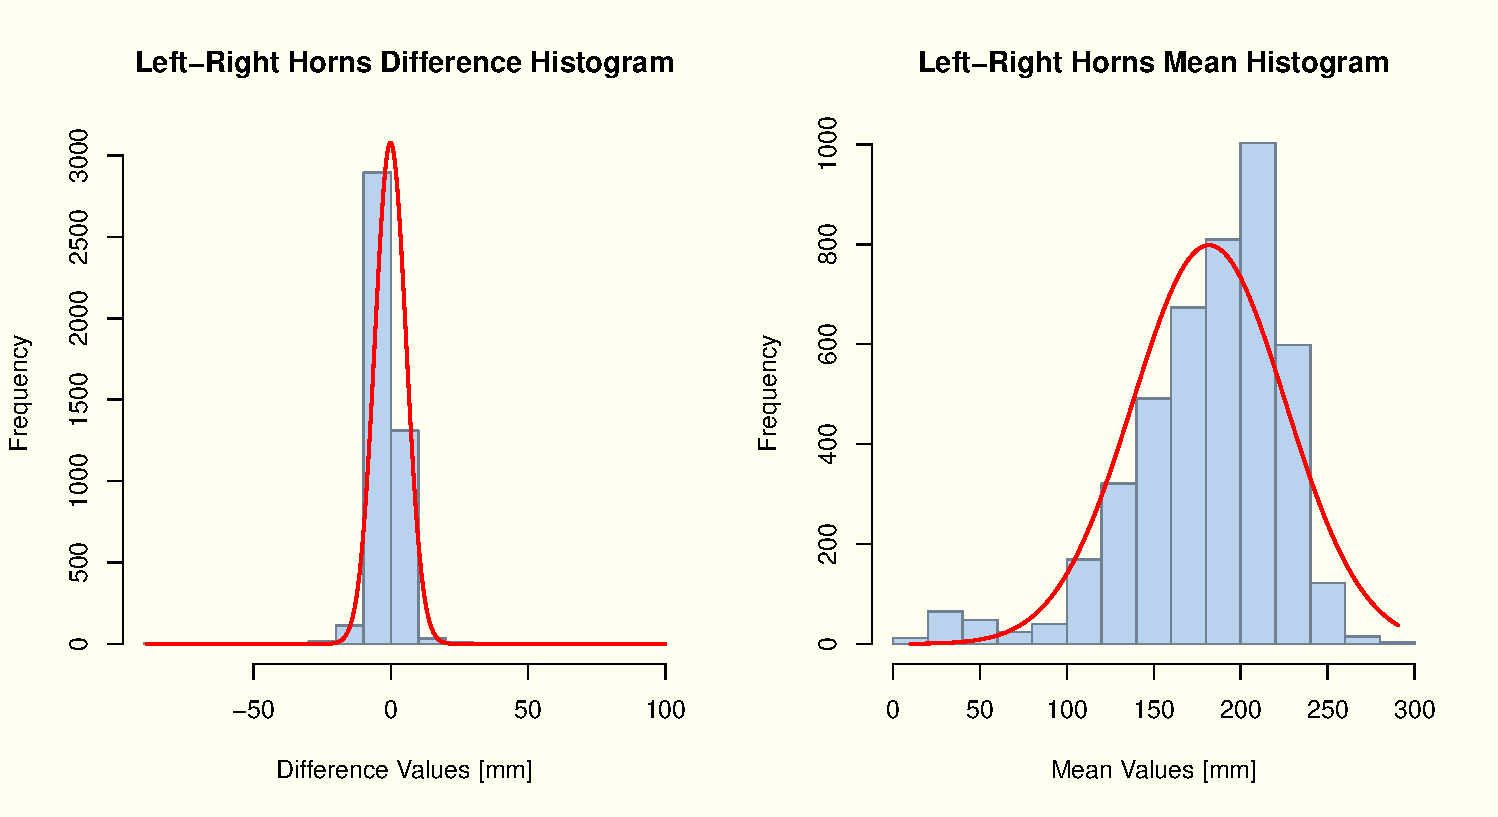
\includegraphics[scale=0.5]{histograms.pdf}
\caption{On the left, the histogram containing in the x-axis the difference between the measurement of the length of the left horn and the right one and their frequency on the y-axis with a normal distribution overlay. On the right the values of the the mean between the horns on the two sides on the x-axis [mm] vs their frequency and a normal distribution overlay.}
  \label{fig:hist}
\end{figure}

I then checked, with some boxplots, see  \autoref{fig:box1} and \autoref{fig:box2}, how data were distributed to get an idea of the results I might obtain before moving onto the two-way ANOVA analysis itself.
\begin{figure}[H]
     \centering
     \caption{True both for the left image and for the right one: on the left, boxplots showing the data distribution of the chosen response variable depending on the sex of the goat. On the right boxplots showing the data distribution of the same variable depending on the density of population at the birth.}
     \subfloat[][Horn length boxplots]{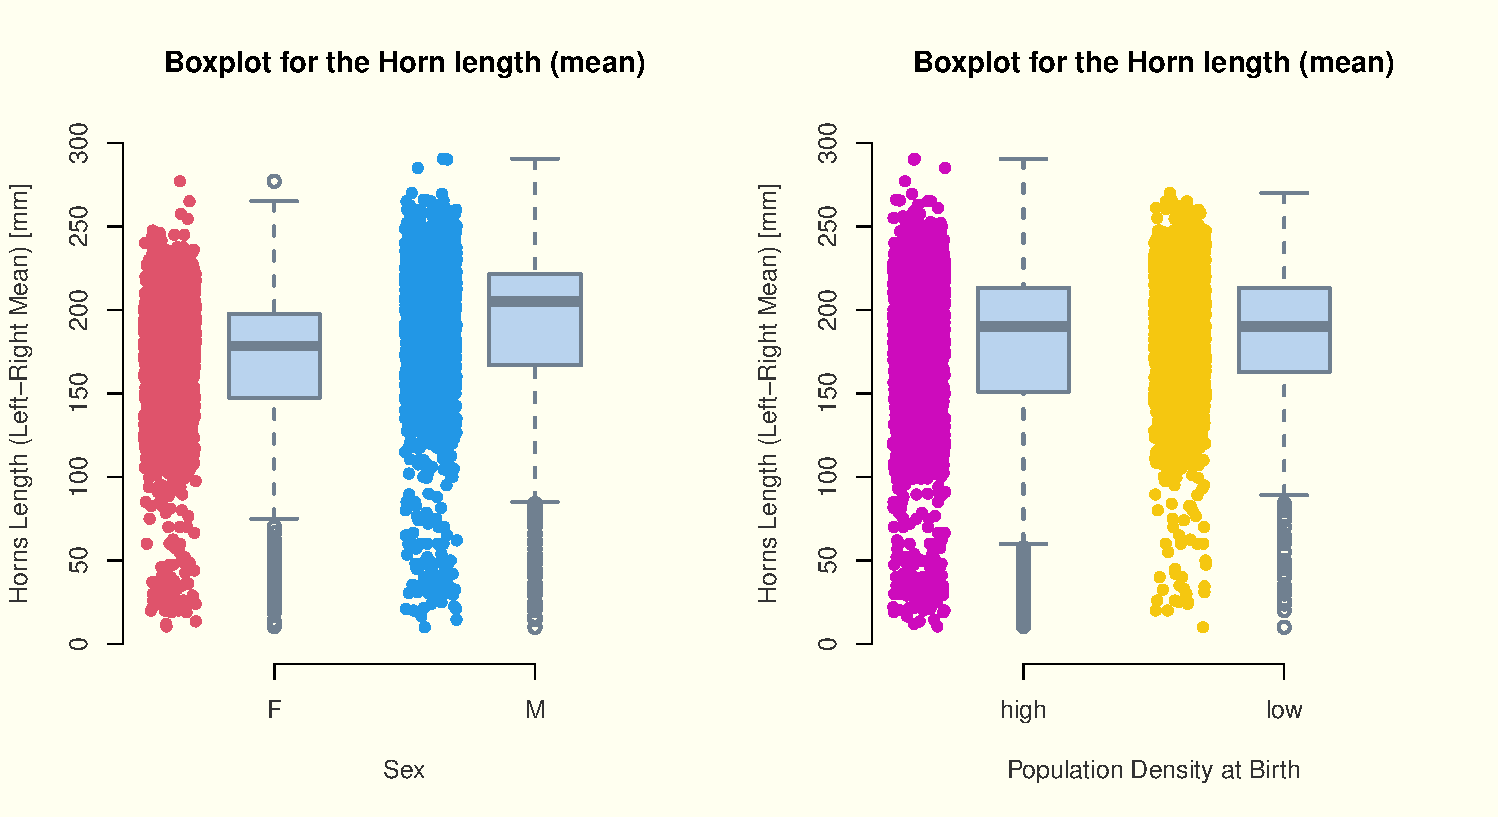
\includegraphics[scale = 0.365]{boxplot-horn.pdf}\label{fig:box1}} \qquad
     \subfloat[][Body mass boxplots]{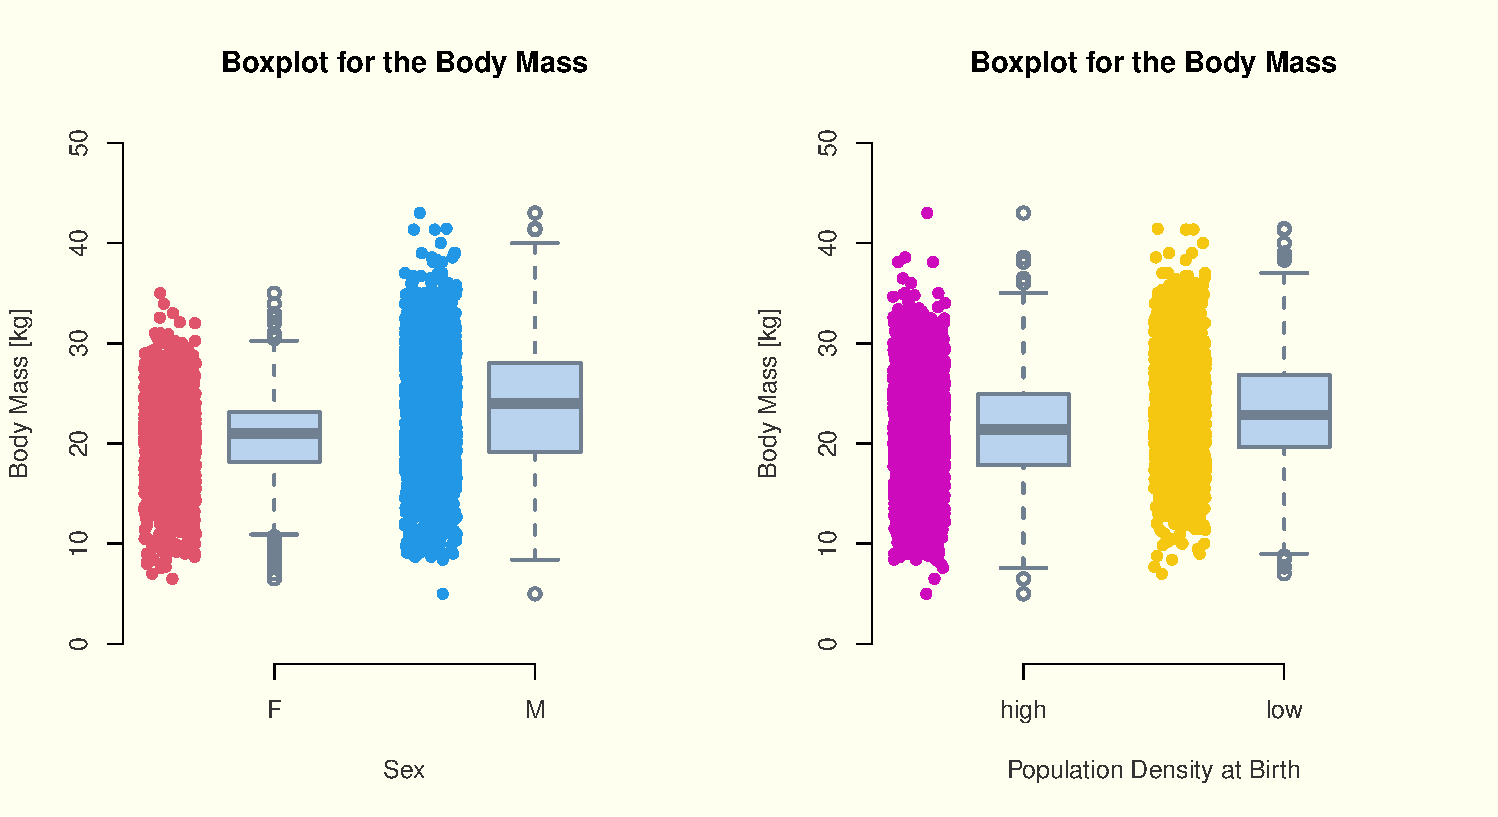
\includegraphics[scale = 0.365]{boxplot-mass.pdf}\label{fig:box2}}
\end{figure}

\iffalse
\begin{figure}[H]
\centering
  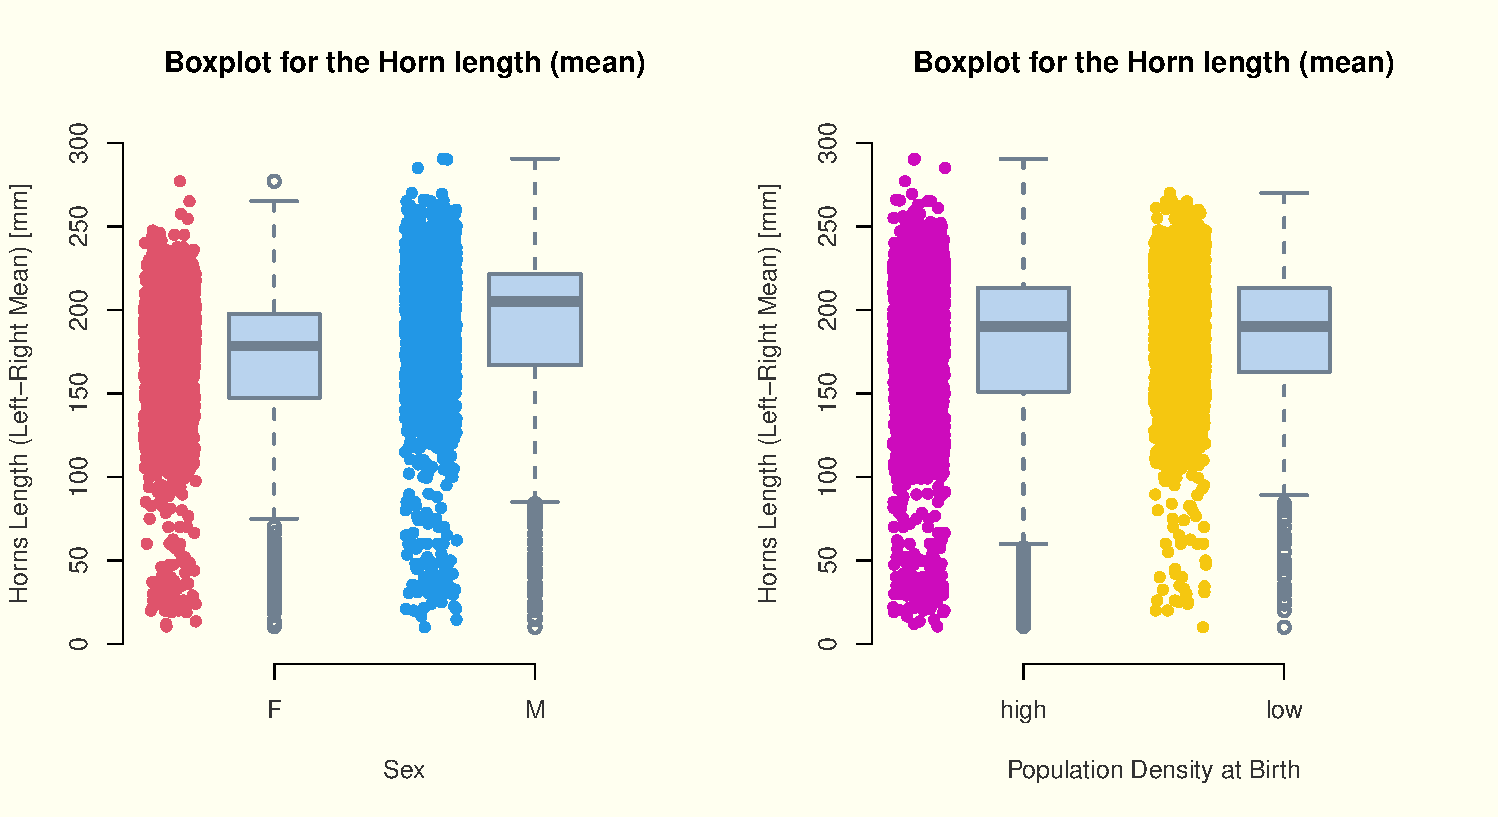
\includegraphics[scale=0.5]{boxplot-horn.pdf}
\caption{On the left, boxplots showing the data distribution of the Horns length (mean between left horn and right horn) depending on the sex of the goat. On the right boxplots showing the data distribution of the Horns length (mean between left horn and right horn) depending on the density of population at the birth.}
  \label{fig:box1}
\end{figure}
\begin{figure}[H]
\centering
  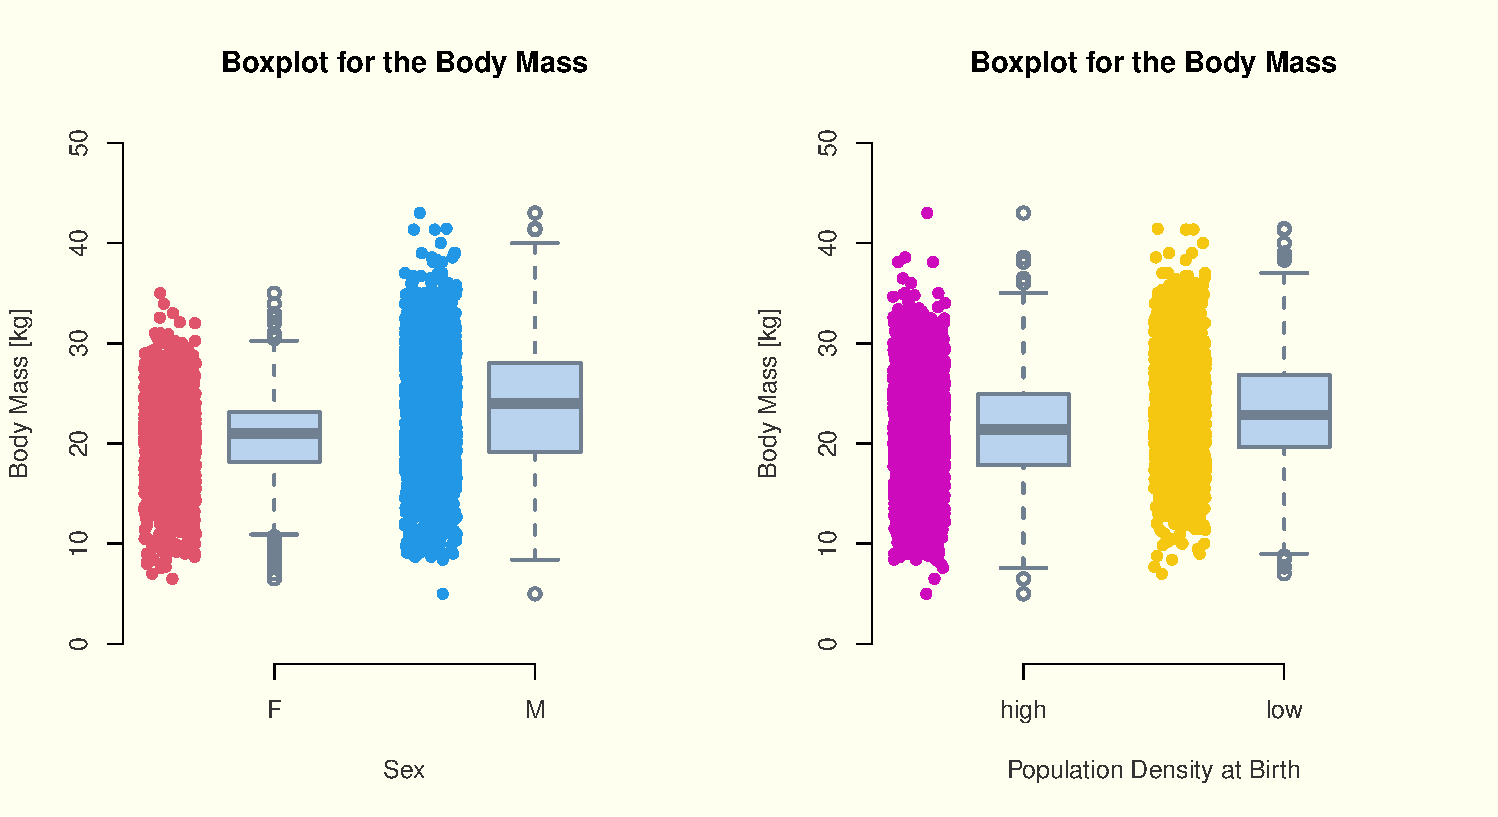
\includegraphics[scale=0.5]{boxplot-mass.pdf}
\caption{On the left, boxplots showing the data distribution of the body mass depending on the sex of the goat. On the right boxplots showing the data distribution of the body mass depending on the density of population at the birth.}
  \label{fig:box2}
\end{figure}
\fi
Now, to get some estimates, I performed the ANOVA analysis. First of all, after summarizing the main values of interest (mean, sd and se for the horns both left and right and for the body mass), \autoref{tab:aov1} and \autoref{tab:aov3}, and next computing the means and errors for the newly created variable "mean\_horns\_lenght", \autoref{tab:A}, from a graphical point of view I obtained \autoref{fig:aov1}.
\begin{table}[H]
\centering
\caption{Summary statistics for the hornL and hornR response variables depending on the two factors.}
\begin{tabular}{c c c c c c c} 
 \hline
Sex & hornL Mean [mm] & hLSD [mm] & hLSE [mm] & hornR Mean [mm] & hRSD [mm] & hRSE [mm]    \\  
 \hline
 Female &169.04&41.32&0.93&169.01&41.19&0.93 \\
 Male &191.91&43.47&0.88&192.20&43.49& 0.88 \\
 \hline
 \hline
 Pop. density & hornL Mean [mm] & hLSD [mm] & hLSE [mm] & hornR Mean [mm] & hRSD [mm] & hRSE [mm]  \\  
 \hline
 High &177.99&48.57&1.02&178.11&48.64&1.02  \\
 Low &185.70&38.23&0.83&185.88&38.14&0.83  \\
 \hline
\end{tabular}
\label{tab:aov1}
\end{table}
\begin{table}[H]
\centering
\caption{Summary statistics for the body mass response variable depending on the two factors.}
\begin{tabular}{c c c c} 
 \hline
Sex & Mass Mean [kg] & Mass SD [kg] & Mass SE [kg]   \\  
 \hline
 Female &20.55&4.05&0.09 \\
 Male &23.67&5.90&0.12  \\
 \hline
 \hline
 Pop. density & Mass Mean [kg] & Mass SD [kg] & Mass SE [kg] \\  
 \hline
 High &21.38&5.33&0.11 \\
 Low &23.23&5.29&0.11  \\
 \hline
\end{tabular}
\label{tab:aov3}
\end{table}
\begin{table}[!htb]
    \caption{Means (above) and standard errors (below) after exploiting the new variable "horn\_mean\_legth" [mm] (on the left side) and body mass [kg] (on the right side).}
    \label{tab:A}
    \begin{minipage}{.5\linewidth}
      \centering
        \begin{tabular}{c c c} 
 \hline
/ & High & Low   \\  
 \hline
 Female &165.12& 173.30\\
 Male &188.72& 195.49  \\
 \hline
 \hline
/ & High & Low   \\  
 \hline
 Female &1.41&1.18 \\
 Male &1.39& 1.06 \\
 \hline
\end{tabular}
    \end{minipage}%
    \begin{minipage}{.5\linewidth}
      \centering
\begin{tabular}{c c c} 
 \hline
/ & High & Low   \\  
 \hline
 Female &19.88&21.29 \\
 Male &22.63&24.74  \\
 \hline
 \hline
/ & High & Low   \\  
 \hline
 Female &0.13&0.12 \\
 Male &0.17&0.17  \\
 \hline
\end{tabular}
    \end{minipage} 
\end{table}
\begin{figure}[H]
\centering
  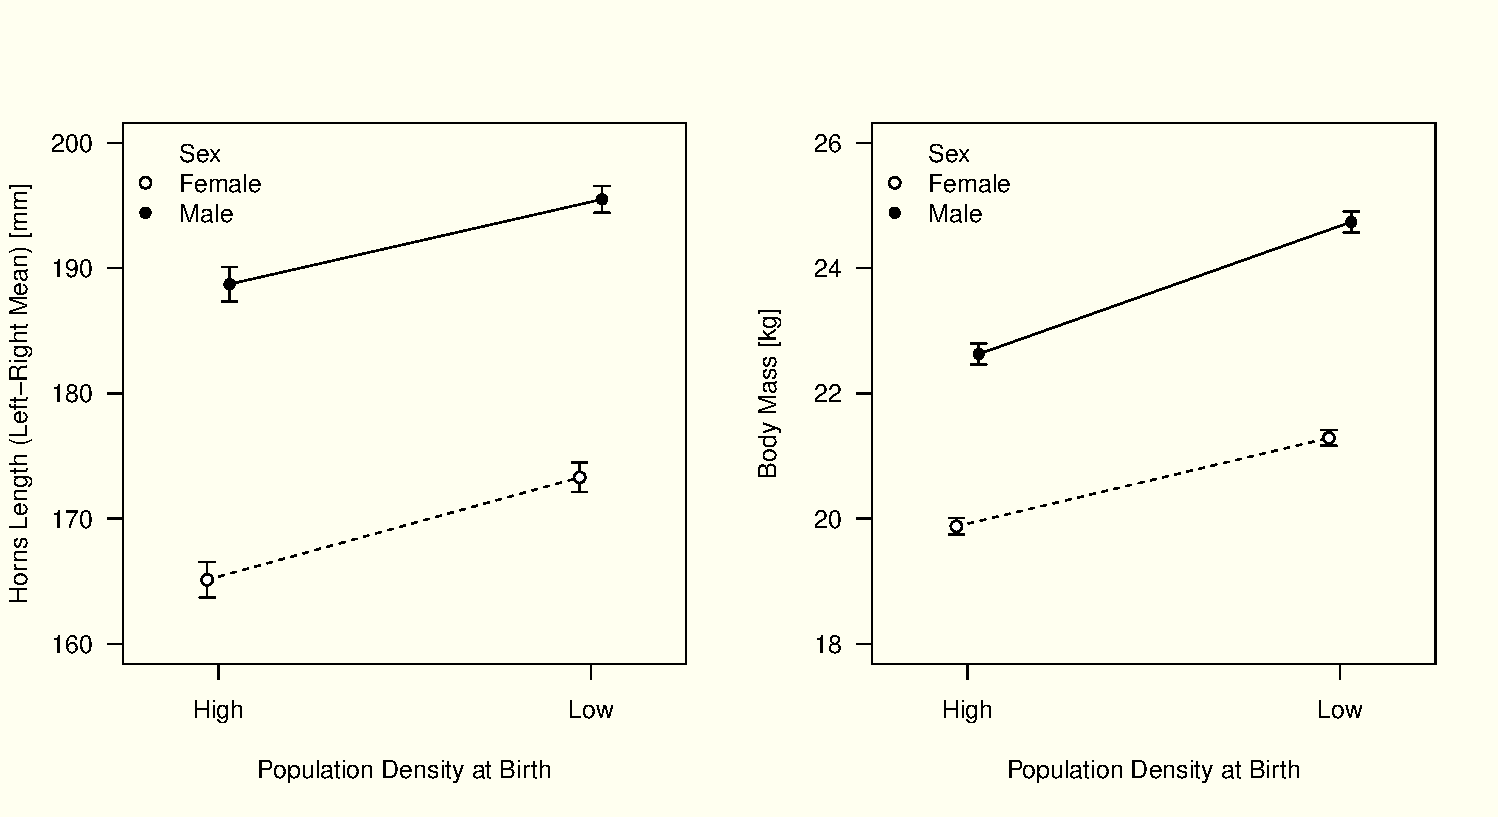
\includegraphics[scale=0.5]{anova2.pdf}
\caption{Plots giving a graphical idea of the size effect for the two-way ANOVA analysis performed for both the horn length and the body mass when considering sex and population density at birth as factors.}
  \label{fig:aov1}
\end{figure}
\iffalse
\begin{table}[H]
\centering
\caption{Means (above) and standard errors (below) after exploiting the new variable "horn\_mean\_legth" [mm].}
\begin{tabular}{c c c} 
 \hline
/ & High & Low   \\  
 \hline
 Female &165.12& 173.30\\
 Male &188.72& 195.49  \\
 \hline
 \hline
/ & High & Low   \\  
 \hline
 Female &1.41&1.18 \\
 Male &1.39& 1.06 \\
 \hline
\end{tabular}
\label{tab:aov2}
\end{table}
\begin{table}[H]
\centering
\caption{Means (above) and standard errors (below) for the variable body mass [kg].}
\begin{tabular}{c c c} 
 \hline
/ & High & Low   \\  
 \hline
 Female &19.88&21.29 \\
 Male &22.63&24.74  \\
 \hline
 \hline
/ & High & Low   \\  
 \hline
 Female &0.13&0.12 \\
 Male &0.17&0.17  \\
 \hline
\end{tabular}
\label{tab:aov4}
\end{table}
\begin{figure}[H]
     \centering
     \subfloat[][text1]{\includegraphics[trim=0 0 1cm 1cm, clip, scale = 0.06]{notube.jpeg}\label{tubeless}} \qquad
     \subfloat[][text2]{\includegraphics[trim=1cm 0 1cm 1cm, clip, scale = 0.1]{tube.jpeg}\label{tube}}
     \caption{caption}
     \label{steady_state}
\end{figure}
\fi

Talking about the horn length (body mass), to interpret the results, by checking first the ANOVA table, one sees that there are detectable effects of both sex and population density, with more variance explained by sex (based on the larger sum of squares: 575479 (10536) and 60026 (3551), respectively).
Furthermore, concerning the horn length only, the effects of sex and population density are independent, as indicated by a negligible statistical support (P > 0.5, F$_{1,4390}$ < 0.4).
Talking about the body mass the effects of sex and population density are, instead, not completely independent as showed by a small statistical support in favor of a small interaction (P $\approx$ 0.02, F$_{1,4390}$ $\approx$ 5).
To quantify the effect size in both cases, I computed the mean horn length and body mass for each population density and sex from \autoref{tab:A} by working first on columns and then on rows. Based on this, I can finally say the following.
The mean horn length (taking the mean between male and female, remembering that I already took the mean between left one and right one in each goat at the beginning as already specified) (body mass) was 4\% shorter (7.6\% smaller) when considering goats born with a high density in population than when having a low population density at birth (mean horn length (body mass) = 176.92 mm (21.25 kg) and 184.39 mm (23.01 kg), respectively, F$_{1,4390}$ = 33.62 (137.62), P << 0.00001, \autoref{fig:aov1}).
When considering the effect of sex, instead, the mean horn length for females (taking the mean between high density and low density after I took the mean between left one and right one in each goat at the beginning as already specified) (body mass) was 12\% shorter (13.1\% lower) with respect to males (mean horn length (body mass) = 169.21 mm (20.58 kg) and 192.10 mm (23.68 kg), respectively, F$_{1,4390}$ = 322.28 (408.31), P << 0.00001, \autoref{fig:aov1}).
The difference in horns length between population densities was very very small between males and females as correctly showed by the negligible above mentioned statistical support for the contribution of the interaction term (3.5\% vs. 4.7\%, respectively; P = 0.58). 
\iffalse
The mean body mass was 7.6\% smaller when considering goats born with a high density in population than when having a low population density at birth (mean body mass = 21.25 and 23.01 kg, respectively, F$_{1,4390}$ = 137.62, P << 0.00001, \autoref{fig:aov1}).
When considering the effect of sex instead, the mean body mass for females (taking the mean between high density and low density) was 13.1\% lower with respect to males (mean body mass = 20.58 and 23.68 kg, respectively, F$_{1,4390}$ = 408.31, P << 0.00001, \autoref{fig:aov1}).
\fi
There was a slight difference in body mass between population densities between males and females as can also be seen by the small but present statistical support in favor of the interaction term in this case (8.5\% vs. 6.6\%, respectively; P = 0.02).
All things considered, from the analysis of this particular dataset with the specified methods, it has been shown that sex is affecting more the horn length and the body mass (both higher in males) of mountain goats compared to the low population densities at birth. No strong interaction has been found between sex and the population density at birth even though a non-negligible statistical support in favor of a small interaction has been outlined when it comes to the body mass response variable.

\iffalse
\AtNextBibliography{\footnotesize}
\printbibliography
\fi
\section{Appendix} \label{Appendix}
The R code used for the analysis of the two datasets is inserted here below.
\subsection{Blossoms in Greenhouse}

\begin{minted}[breaklines,frame=single]{R}
library(sciplot)
library(magrittr) 
library(dplyr)    
library(plyr)
library(knitr)
library(rcompanion)
library(MASS)

################################################################################
################################################################################
#
# DATASET INTRODUCTION AS USUAL
#
################################################################################
################################################################################

dat = read.csv("exam2022_part1.csv")
head(dat)
names(dat)
View(dat)
str(dat)
dat = na.omit(dat)
############################
# creation of sub-datasets
############################

dat_wet = dat[dat$treat=="W",]
dat_dry = dat[dat$treat=="D",]
dat_S = dat[dat$sp=="S",]
dat_L = dat[dat$sp=="L",]

View(dat_wet)
View(dat_dry)
View(dat_S)
View(dat_L)
################################################################################
# VARIABLES ORGANIZING AND CHECKING PLUS HISTOGRAMS 
################################################################################

populations = as.factor(dat$pop)
species = as.factor(dat$sp)
treatment = as.factor(dat$treat)

################################################################
# checking LBL and UBL with histograms for each dataset
################################################################


##############################################################################
##############################################################################
#
# 4x4 histograms for LBL for the various subdataset
#
##############################################################################
##############################################################################

par(mfrow=c(2,2))
par(bg = "ivory")

plotNormalHistogram(dat_wet$LBL, prob = FALSE, col="slategray2", border="slategray",xlim = c(10,32),
                    main = "LBL (wet only) Normal Overlay on Histogram", xlab = "LBL [mm]",
                    linecol="red", lwd=2 )
plotNormalHistogram(dat_L$LBL, prob = FALSE, col="slategray2", border="slategray",
                    main = "LBL (L-species) Normal Overlay on Histogram", xlab = "LBL [mm]",
                    linecol="red", lwd=2 )
plotNormalHistogram(dat_dry$LBL, prob = FALSE, col="slategray2", border="slategray",xlim = c(10,32),
                    main = "LBL (dry only) Normal Overlay on Histogram", xlab = "LBL [mm]",
                    linecol="red", lwd=2 )
plotNormalHistogram(dat_S$LBL, prob = FALSE, col="slategray2", border="slategray",
                    main = "LBL (S-species) Normal Overlay on Histogram", xlab = "LBL [mm]",
                    linecol="red", lwd=2)

par(oldpar)

##############################################################################
##############################################################################
#
# 4x4 histograms for UBL for the various subdataset
#
##############################################################################
##############################################################################

par(mfrow=c(2,2))
par(bg = "ivory")
plotNormalHistogram(dat_wet$UBL, prob = FALSE, col="slategray2", border="slategray",xlim = c(10,30),
                    main = "UBL (wet only) Normal Overlay on Histogram", xlab = "UBL [mm]",
                    linecol="red", lwd=2 )
plotNormalHistogram(dat_L$UBL, prob = FALSE, col="slategray2", border="slategray",
                    main = "UBL (L-species) Normal Overlay on Histogram", xlab = "UBL [mm]",
                    linecol="red", lwd=2 )
plotNormalHistogram(dat_dry$UBL, prob = FALSE, col="slategray2", border="slategray",xlim = c(10,30),
                    main = "UBL (dry only) Normal Overlay on Histogram", xlab = "UBL [mm]",
                    linecol="red", lwd=2 )
plotNormalHistogram(dat_S$UBL, prob = FALSE, col="slategray2", border="slategray",
                    main = "UBL (S-species) Normal Overlay on Histogram", xlab = "UBL [mm]",
                    linecol="red", lwd=2)
par(oldpar)

##############################################################################
##############################################################################
#
# Doing boxplots to visualize data of UBL and LBL
#
##############################################################################
##############################################################################

########
# dat
########

########
# first LBL
########

par(mfrow=c(1,2))
par(bg = "ivory")
boxplot(dat$LBL~species, xlab="Species", ylim = c(9, 35),
        ylab="LBL [mm]",boxwex=0.35, main = "Boxplot of LBL data for species", lwd = 2, border= "slategrey", # colour of the box borders
        col = "slategray2", # colour of the inside of the boxes
        col.axis = 'grey20', # colour of the axis numbers 
        col.lab = 'grey20', # colour of the axis labels
        frame = F)
stripchart(dat$LBL~species,
           method = "jitter",  main = "method = 'jitter', jitter = 0.2",
           pch = 16, # specify the type of point to use
           cex = 1,
           col = c(3,2),
           vertical = TRUE, 
           at = c(0.6,1.6),
           add = TRUE)
# at = c(0.75,1.75)

boxplot(dat$LBL~treatment, xlab="Treatments", ylim = c(9, 35),
        ylab="LBL [mm]",boxwex=0.35, main = "Boxplot of LBL data for treatments", lwd = 2, border= "slategrey", # colour of the box borders
        col = "slategray2", # colour of the inside of the boxes
        col.axis = 'grey20', # colour of the axis numbers 
        col.lab = 'grey20', # colour of the axis labels
        frame = F)
stripchart(dat$LBL~treatment,
           method = "jitter",  main = "method = 'jitter', jitter = 0.2",
           pch = 16, # specify the type of point to use
           cex = 1,
           col = c(7,4),
           vertical = TRUE, 
           at = c(0.6,1.6),
           add = TRUE)

par(oldpar)

########
# now UBL
########


par(mfrow=c(1,2))
par(bg = "ivory")
boxplot(dat$UBL~species, xlab="Species", ylim = c(8, 30),
        ylab="UBL [mm]",boxwex=0.35, main = "Boxplot of UBL data for species", lwd = 2, border= "slategrey", # colour of the box borders
        col = "slategray2", # colour of the inside of the boxes
        col.axis = 'grey20', # colour of the axis numbers 
        col.lab = 'grey20', # colour of the axis labels
        frame = F)
stripchart(dat$UBL~species,
           method = "jitter",  main = "method = 'jitter', jitter = 0.2",
           pch = 16, # specify the type of point to use
           cex = 1,
           col = c(3,2),
           vertical = TRUE, 
           at = c(0.6,1.6),
           add = TRUE)
# at = c(0.75,1.75)

boxplot(dat$UBL~treatment, xlab="Treatments", ylim = c(8, 30),
        ylab="UBL [mm]",boxwex=0.35, main = "Boxplot of UBL data for treatments", lwd = 2, border= "slategrey", # colour of the box borders
        col = "slategray2", # colour of the inside of the boxes
        col.axis = 'grey20', # colour of the axis numbers 
        col.lab = 'grey20', # colour of the axis labels
        frame = F)
stripchart(dat$UBL~treatment,
           method = "jitter",  main = "method = 'jitter', jitter = 0.2",
           pch = 16, # specify the type of point to use
           cex = 1,
           col = c(7,4),
           vertical = TRUE, 
           at = c(0.6,1.6),
           add = TRUE)

par(oldpar)

##############################################################################
##############################################################################
#
# end of boxplots to visualize data
#
##############################################################################
##############################################################################



################################################################################
# 2-WAY ANOVA FOR HORNS LENGTH For UBL and LBL with factors treatment and species
################################################################################


################################################################################
# STARTING THE FIRST 2-WAY ANOVA FOR LBL
################################################################################

means = tapply(dat$LBL, list(species, treatment), mean)
ses = tapply(dat$LBL,
             list(species, treatment),
             function(x) sd(x)/sqrt(sum(!is.na(x))))
means
ses

m = lm(dat$LBL~species*treatment)
anova(m)
summary(m)
colMeans(means)
rowMeans(means)


################################################################################
# SECOND 2-WAY ANOVA FOR UBL
################################################################################

means2 = tapply(dat$UBL, list(species, treatment), mean)
ses2 = tapply(dat$UBL,
              list(species, treatment),
              function(x) sd(x)/sqrt(sum(!is.na(x))))
means2
ses2

m3 = lm(dat$UBL~species*treatment)
anova(m3)
summary(m3)
colMeans(means2)
rowMeans(means2)


################################################################################
# PUTTING PLOTS TOGETHER
################################################################################

par(mfrow=c(1,2))
par(bg = "ivory")

plot(c(0.97, 1.03), means[,1], ylim=c(14, 25), xlim=c(0.8, 2.2),
     xlab="Treatment",
     ylab="Lower Bract Length (LBL) [mm]",
     xaxt="n", las=1, pch=c(21,16), col="white")
axis(1, 1:2, labels=c("Dry", "Wet"))
arrows(c(0.97,1.03), means[,1]-ses[,1], c(0.97,1.03),
       means[,1]+ses[,1], length=0.05, angle=90, code=3)
arrows(c(1.97,2.03), means[,2]-ses[,2], c(1.97,2.03),
       means[,2]+ses[,2], length=0.05, angle=90, code=3)
segments(0.97, means[1,1], 1.97, means[1,2], lty=2)
segments(1.03, means[2,1], 2.03, means[2,2])
points(c(0.97, 1.03), means[,1], pch=c(21,16), bg="white")
points(c(1.97, 2.03), means[,2], pch=c(21, 16), bg="white")
legend("topleft", c("Species", "L", "S"),
       bty="n", pch=c(NA,21,16))

plot(c(0.97, 1.03), means2[,1], ylim=c(14, 25), xlim=c(0.8, 2.2),
     xlab="Treatment",
     ylab="Upper Bract Length (UBL) [mm]",
     xaxt="n", las=1, pch=c(21,16), col="white")
axis(1, 1:2, labels=c("Dry", "Wet"))
arrows(c(0.97,1.03), means2[,1]-ses2[,1], c(0.97,1.03),
       means2[,1]+ses2[,1], length=0.05, angle=90, code=3)
arrows(c(1.97,2.03), means2[,2]-ses2[,2], c(1.97,2.03),
       means2[,2]+ses2[,2], length=0.05, angle=90, code=3)
segments(0.97, means2[1,1], 1.97, means2[1,2], lty=2)
segments(1.03, means2[2,1], 2.03, means2[2,2])
points(c(0.97, 1.03), means2[,1], pch=c(21,16), bg="white")
points(c(1.97, 2.03), means2[,2], pch=c(21, 16), bg="white")
legend("topleft", c("Species", "L", "S"),
       bty="n", pch=c(NA,21,16))


par(oldpar)

\end{minted}

\subsection{Mountain Goats}
\begin{minted}[breaklines,frame=single]{R}
library(sciplot)
library(magrittr) 
library(dplyr)    
library(plyr)
library(knitr)
library(rcompanion)
library(MASS)

################################################################################
################################################################################
#
# DATASET INTRODUCTION AS USUAL
#
################################################################################
################################################################################

dat = read.table("exam2022_part2.txt", header=T) 
head(dat)
names(dat)
View(dat)
str(dat)
dat = na.omit(dat)

################################################################################
# VARIABLES ORGANIZING AND CHECKING PLUS HISTOGRAMS 
################################################################################

sex = as.factor(dat$sex)
density = as.factor(dat$density)
#plot(dat)
horns_difference = dat$hornL - dat$hornR
mean_horns_lenght = (dat$hornL + dat$hornR)/2


oldpar = par(no.readonly = TRUE)


par(mfrow=c(1,2))
par(bg = "ivory")

plotNormalHistogram(horns_difference, prob = FALSE, col="slategray2", border="slategray",
                    main = "Left-Right Horns Difference Histogram", xlab = "Difference Values [mm]",
                    linecol="red", lwd=2 )


plotNormalHistogram(mean_horns_lenght, prob = FALSE, col="slategray2", border="slategray",
                    main = "Left-Right Horns Mean Histogram", xlab = "Mean Values [mm]",
                    linecol="red", lwd=2 )

par(oldpar)


fitdistr(horns_difference, "normal")


fitdistr(mean_horns_lenght, "normal")

# sex as categorical variable

popstats = ddply(dat, .(sex), summarize,
                  hornLm = mean(hornL, na.rm=T),
                  hornLsd = sd(hornL, na.rm=T),
                  hornLse = se(hornL, na.rm=T),
                  hornRm = mean(hornR, na.rm=T),
                  hornRsd = sd(hornR, na.rm=T),
                  hornRse = se(hornR, na.rm=T),
                  massm = mean(mass, na.rm=T),
                  masssd = sd(mass, na.rm=T),
                  massse = se(mass, na.rm=T))
popstats[,-1] = round(popstats[,-1], 2)
kable(popstats)

# population density at birth as categorical variable

popstats2 = ddply(dat, .(density), summarize,
                  hornLm = mean(hornL, na.rm=T),
                  hornLsd = sd(hornL, na.rm=T),
                  hornLse = se(hornL, na.rm=T),
                  hornRm = mean(hornR, na.rm=T),
                  hornRsd = sd(hornR, na.rm=T),
                  hornRse = se(hornR, na.rm=T),
                  massm = mean(mass, na.rm=T),
                  masssd = sd(mass, na.rm=T),
                  massse = se(mass, na.rm=T))
popstats2[,-1] = round(popstats2[,-1], 2)
kable(popstats2)
################################################################################
# TOWARDS 2-WAY ANOVA: LOOKING AT BOXPLOTS
################################################################################

oldpar = par(no.readonly = TRUE)


par(mfrow=c(1,2))
par(bg = "ivory")
boxplot(mean_horns_lenght~sex, xlab="Sex", ylim = c(0, 300),
        ylab="Horns Length (Left-Right Mean) [mm]",boxwex=0.35, main = "Boxplot for the Horn length (mean)", lwd = 2, border= "slategrey", # colour of the box borders
        col = "slategray2", # colour of the inside of the boxes
        col.axis = 'grey20', # colour of the axis numbers 
        col.lab = 'grey20', # colour of the axis labels
        frame = F)
stripchart(mean_horns_lenght~sex,
           method = "jitter",  main = "method = 'jitter', jitter = 0.2",
           pch = 16, # specify the type of point to use
           cex = 1,
           col = c(2,4),
           vertical = TRUE,
           at = c(0.6,1.6),
           add = TRUE)


boxplot(mean_horns_lenght~density, xlab="Population Density at Birth", ylim = c(0, 300),
        ylab="Horns Length (Left-Right Mean) [mm]",boxwex=0.35, main = "Boxplot for the Horn length (mean)", lwd = 2, border= "slategrey", # colour of the box borders
        col = "slategray2", # colour of the inside of the boxes
        col.axis = 'grey20', # colour of the axis numbers 
        col.lab = 'grey20', # colour of the axis labels
        frame = F)
stripchart(mean_horns_lenght~density,
           method = "jitter",  main = "method = 'jitter', jitter = 0.2",
           pch = 16, # specify the type of point to use
           cex = 1,
           col = c(6,7),
           vertical = TRUE, 
           at = c(0.6,1.6),
           add = TRUE)


par(oldpar)



par(mfrow=c(1,2))
par(bg = "ivory")


boxplot(dat$mass~sex, xlab="Sex", ylim = c(0, 50),
        ylab="Body Mass [kg]",boxwex=0.35, main = "Boxplot for the Body Mass", lwd = 2, border= "slategrey", # colour of the box borders
        col = "slategray2", # colour of the inside of the boxes
        col.axis = 'grey20', # colour of the axis numbers 
        col.lab = 'grey20', # colour of the axis labels
        frame = F)
stripchart(dat$mass~sex,
           method = "jitter",  main = "method = 'jitter', jitter = 0.2",
           pch = 16, # specify the type of point to use
           cex = 1,
           col = c(2,4),
           vertical = TRUE,
           at = c(0.6,1.6),
           add = TRUE)


boxplot(dat$mass~density, xlab="Population Density at Birth", ylim = c(0, 50),
        ylab="Body Mass [kg]",boxwex=0.35, main = "Boxplot for the Body Mass", lwd = 2, border= "slategrey", # colour of the box borders
        col = "slategray2", # colour of the inside of the boxes
        col.axis = 'grey20', # colour of the axis numbers 
        col.lab = 'grey20', # colour of the axis labels
        frame = F)
stripchart(dat$mass~density,
           method = "jitter",  main = "method = 'jitter', jitter = 0.2",
           pch = 16, # specify the type of point to use
           cex = 1,
           col = c(6,7),
           vertical = TRUE, 
           at = c(0.6,1.6),
           add = TRUE)
par(oldpar)
################################################################################
# STARTING THE FIRST 2-WAY ANOVA FOR HORNS LENGTH
################################################################################

means = tapply(mean_horns_lenght, list(sex, density), mean)
ses = tapply(mean_horns_lenght,
             list(sex, density),
             function(x) sd(x)/sqrt(sum(!is.na(x))))
means
ses


m = lm(mean_horns_lenght~sex*density)
anova(m)
summary(m)
colMeans(means)
rowMeans(means)


################################################################################
# SECOND 2-WAY ANOVA FOR BODY MASS
################################################################################

means2 = tapply(dat$mass, list(sex, density), mean)
ses2 = tapply(dat$mass,
             list(sex, density),
             function(x) sd(x)/sqrt(sum(!is.na(x))))
means2
ses2


m3 = lm(dat$mass~sex*density)
anova(m3)
summary(m3)
colMeans(means2)
rowMeans(means2)


################################################################################
# PUTTING PLOTS TOGETHER
################################################################################

par(mfrow=c(1,2))
par(bg = "ivory")

plot(c(0.97, 1.03), means[,1], ylim=c(160, 200), xlim=c(0.8, 2.2),
     xlab="Population Density at Birth",
     ylab="Horns Length (Left-Right Mean) [mm]",
     xaxt="n", las=1, pch=c(21,16), col="white")
axis(1, 1:2, labels=c("High", "Low"))
arrows(c(0.97,1.03), means[,1]-ses[,1], c(0.97,1.03),
       means[,1]+ses[,1], length=0.05, angle=90, code=3)
arrows(c(1.97,2.03), means[,2]-ses[,2], c(1.97,2.03),
       means[,2]+ses[,2], length=0.05, angle=90, code=3)
segments(0.97, means[1,1], 1.97, means[1,2], lty=2)
segments(1.03, means[2,1], 2.03, means[2,2])
points(c(0.97, 1.03), means[,1], pch=c(21,16), bg="white")
points(c(1.97, 2.03), means[,2], pch=c(21, 16), bg="white")
legend("topleft", c("Sex", "Female", "Male"),
       bty="n", pch=c(NA,21,16))

plot(c(0.97, 1.03), means2[,1], ylim=c(18, 26), xlim=c(0.8, 2.2),
     xlab="Population Density at Birth",
     ylab="Body Mass [kg]",
     xaxt="n", las=1, pch=c(21,16), col="white")
axis(1, 1:2, labels=c("High", "Low"))
arrows(c(0.97,1.03), means2[,1]-ses2[,1], c(0.97,1.03),
       means2[,1]+ses2[,1], length=0.05, angle=90, code=3)
arrows(c(1.97,2.03), means2[,2]-ses2[,2], c(1.97,2.03),
       means2[,2]+ses2[,2], length=0.05, angle=90, code=3)
segments(0.97, means2[1,1], 1.97, means2[1,2], lty=2)
segments(1.03, means2[2,1], 2.03, means2[2,2])
points(c(0.97, 1.03), means2[,1], pch=c(21,16), bg="white")
points(c(1.97, 2.03), means2[,2], pch=c(21, 16), bg="white")
legend("topleft", c("Sex", "Female", "Male"),
       bty="n", pch=c(NA,21,16))

par(oldpar)

\end{minted}
\end{document}
